\documentclass[11pt,a4paper]{article}

% --- Mathematics (must precede unicode-math) ---
\usepackage{amsmath}
\usepackage{mathtools}

% --- Fonts (lualatex) ---
\usepackage{fontspec}
\usepackage{unicode-math}
\setmathfont{KpMath-Regular.otf}
\setmathfont{KpMath-Bold.otf}[version=bold]

\usepackage{microtype}
\usepackage[dvipsnames]{xcolor}
\usepackage[margin=25mm, top=30mm, bottom=30mm]{geometry}

\usepackage{fancyhdr}
\pagestyle{fancy}
\fancyhf{}
\fancyhead[L]{\small\itshape A Cartesian Multipole Hierarchy for the Voxel}
\fancyhead[R]{\small\itshape Nestor (2026)}
\fancyfoot[C]{\thepage}
\renewcommand{\headrulewidth}{0.4pt}
\renewcommand{\footrulewidth}{0pt}

\setcounter{secnumdepth}{3}
\usepackage{booktabs}
\usepackage{array}
\usepackage{graphicx}
\usepackage{placeins}
\usepackage[numbers,sort&compress]{natbib}
\usepackage[font=small, labelfont=bf, labelsep=period]{caption}
\usepackage{setspace}
\setstretch{1.15}
\setlength{\parskip}{0.4em}
\usepackage[colorlinks=true, linkcolor=blue!60!black,
            citecolor=blue!60!black, urlcolor=blue!60!black]{hyperref}

% --- Macros ---
\newcommand{\bI}{\mathbf{I}}
\newcommand{\bA}{\mathbf{A}}
\newcommand{\bS}{\mathbf{S}}
\newcommand{\bT}{\mathbf{T}}
\newcommand{\bK}{\mathbf{K}}
\newcommand{\bP}{\mathbf{P}}
\newcommand{\bD}{\boldsymbol{\Delta}}
\newcommand{\bG}{\mathbf{G}}
\newcommand{\sinc}{\operatorname{sinc}}
\newcommand{\nb}[1]{\texttt{#1}}
% the differential of every integral and derivative is upright: \dd z, \dd^2x, \frac{\dd}{\dd z};
% an italic d is the lattice pitch. JCP/make_jcp.py refuses to build if this is broken.
\newcommand{\dd}{\mathrm{d}}

\title{\bfseries A Cartesian Multipole Hierarchy for the Voxel\\[4pt]
\large Closed-Form Single-Site $T$-Matrices of an Elastic Cube}
\author{T. M. Nestor\\[2pt]\small Independent researcher, Australia}
\date{Draft, 9 October 2026}

\begin{document}
\maketitle

\begin{abstract}
\noindent
Volume-integral (coupled-dipole) methods divide a heterogeneous elastic medium into cubic voxels, each
carrying a single-site $T$-matrix, coupled through the Green's tensor of a background medium. The single
site is usually imported: from the ellipsoid, for which Eshelby's uniformity theorem holds, or from a
polarisability tuned to a lattice. We derive it instead, as the first member of a Cartesian multipole
hierarchy: each voxel radiates through the Cartesian multipole moments of its source and receives the
field through its gradients at its centre, the integrals over the source cube being exact at every
separation, so that touching voxels and the self term, a distribution in closed form, are included and
there is no radius of convergence. Its coefficients are moments of the elastodynamic Green's tensor over
the cube, in closed form on four constants, and nothing in it is fitted. At the order of the
uniform-strain closure a cube is a sphere plus a pure cubic anisotropy, which splits the deviatoric
channel about the sphere's value in the ratio $3:2$, and the closure departs from exact scattering by a
sphere only through a real term of order $(ka)^2$, the radiation damping agreeing exactly. Its blocks gain
accuracy in parity pairs, with the error of each truncation in closed form: with third gradients the
single site is three hundred times more accurate than the uniform-strain closure against the exact sphere,
and as a voxel scheme the hierarchy is fourth order on a smoothly graded sphere. Every result is derived
symbolically and checked against an independent implementation or an exact solution.
\end{abstract}

\section{Introduction}\label{sec:intro}

\paragraph{The problem this paper serves.} Seismic waves in the crust are scattered by heterogeneity
on every scale, and the aim of the work this paper begins is an efficient model of the wavefield in a
medium of realistic complication. The models that describe such a medium are parameterised in many
ways (as layers or blocks, by smooth basis functions, or by interfaces), and a calculation that uses
one must first sample it onto a grid. A volume-integral scattering calculation divides the medium into
cells and treats every cell as a scatterer: a voxel carrying a single-site $T$-matrix, the operator
that turns the field incident on the voxel into the sources it radiates, and coupled to every other
voxel through the Green's tensor of the background, with the multiple-scattering series summed.


\paragraph{The question: the single site.} A voxel is a small region in which two functions must be
represented, the medium and the wavefield, and its single-site $T$-matrix is the operator that turns the
field incident on it into the sources it radiates. Which bases those two functions need, and what error a
given choice leaves, is the subject of a companion paper \citep{NestorError2026}, which isolates the error
exactly on a layer of voxels and finds that every error of the scheme is made at the single site: the
coupling between cubes that tile space, averaged over the source cell, is the continuum's cell integral
exactly. The single site is therefore the object to get right. This paper derives it rather than importing
it, and states the error of each approximation to it.

\paragraph{The coupled-dipole method.} Replacing a heterogeneous body by a lattice of small
scatterers that interact through the background Green's function is the multiple-scattering
description of \citet{Foldy1945} and \citet{Lax1951}. In electromagnetics it became a numerical
method as the coupled-dipole method, or discrete dipole approximation (DDA): each cell of a cubic
grid is a polarisable point dipole driven by the incident field and by the fields of every other
dipole \citep{Purcell1973,Draine1994}. The method is a collocation of the volume integral equation
for the electric field, with the cell's self-interaction absorbed into its polarisability
\citep{Lakhtakia1992}, and \citet{YurkinHoekstra2007} review it in that form. Its accuracy turns on
two ingredients. This paper takes up the first for elasticity; the second is taken up in the companion
paper \citep{NestorError2026}. The first is the polarisability. The
Clausius--Mossotti value is the static response of a sphere; the lattice dispersion relation of
\citet{Draine1993} adjusts it so that an infinite lattice propagates waves as the continuum does to
a given order in $kd$; \citet{Rahmani2002} instead derive it from the exact static solution for the
whole body, so that the method is exact in the long-wavelength limit. The second is the coupling.
Integrating the Green tensor over the source cell rather than sampling it at the centre improves the
accuracy, most of all for strong contrasts \citep{Chaumet2004}, and the filtered coupled dipoles of
\citet{Piller1998}, revived by \citet{Yurkin2010} for large refractive indices, replace the point
dipole by a source of finite extent whose spectrum is band-limited to the grid. The coupling summed
over a lattice extends the method to periodic structures \citep{Chaumet2003}. Its error converges
at second order in the dipole spacing when shape errors are absent \citep{Yurkin2006}, and for a
cube, the one shape a cubic grid represents without a staircase, \citet{YurkinKahnert2013} reach
relative uncertainties of $10^{-7}$ to $10^{-3}$ by extrapolation in the grid. On the mathematical
side, \citet{Costabel2023} show that the method is a finite section of an infinite block Toeplitz
matrix, stable for a large range of the contrast but not for all of it, and \citet{Costabel2023Hilbert}
that in a one-dimensional model it converges at second order in the interior, with a boundary layer in
which the consistency error does not vanish. What this paper adds is the single site in closed form:
for a cube, the polarisability is neither tuned nor imported but derived, from the moments of the
elastodynamic Green's tensor over the cube, with the error of each truncation stated. In the terms of
\citet{NestorError2026} the coupled-dipole method is the voxel of degree zero, and its refinements
improve the polarisability and the coupling while leaving the internal field uniform.

\paragraph{Its elastic counterparts.} The elastic problem has the same volume integral equation
\citep{Gubernatis1977}, and every cell-based solver of it is a coupled-dipole method whether or not
it carries the name. \citet{Nestor1996} divided a two-and-a-half-dimensional medium into cells that
interact through the background Green's tensor, each carrying a contrast renormalised by its own
near field, with the multiple-scattering series summed. \citet{Kanaun2013} discretise the inclusion
problem with Gaussian approximating functions whose matrix elements are analytic. \citet{Yang2008}
solve a stress--velocity form of the integral equation on a grid by conjugate gradients with fast
Fourier transforms, and \citet{Touhei2011} does the same for a half space with a generalised Fourier
transform. \citet{Jakobsen2012} and \citet{Jakobsen2020} build the seismic forward and inverse problems on the
transition operator of the discretised Lippmann--Schwinger equation, the first in the acoustic
approximation and the second in arbitrary anisotropic elastic media with a nine-component state vector.


\paragraph{This paper.} It extends the single site of \citet{Nestor1996} to cubic voxels.
\S\ref{sec:setting} sets out the discrete medium and where its kernel comes from. \S\ref{sec:single}
derives the single-site $T$-matrix as the first member of a Cartesian multipole hierarchy in closed form,
and sets out what that gives (\S\ref{sec:whyclosed}). \S\ref{sec:gradvoxel} builds the hierarchy into a
voxel scheme in three dimensions. \S\ref{sec:discussion} discusses the results and \S\ref{sec:summary}
concludes. Every result is derived symbolically in Mathematica and checked against an independent
Python/Fortran implementation or an exact solution.

\section{Setting}\label{sec:setting}

\paragraph{The discrete medium.} Space is tiled by cubes of side $d$ (half-side $h=d/2$). Cube $i$
carries a contrast $\Delta\lambda,\Delta\mu,\Delta\rho$ from an isotropic background with Lamé
parameters $\lambda,\mu$, density $\rho$, P and S speeds $\alpha,\beta$ and P-wave modulus
$M_P=\lambda+2\mu$. Time dependence is $\mathrm{e}^{-\mathrm{i}\omega t}$; $k_P=\omega/\alpha$, $k_S=\omega/\beta$.
Coordinates are ordered $(z,x,y)$ with $z$ down. The field at a voxel is the nine-component state
\begin{equation}
  \psi=(u_z,u_x,u_y,\ \varepsilon_{zz},\varepsilon_{xx},\varepsilon_{yy},
  2\varepsilon_{xy},2\varepsilon_{zy},2\varepsilon_{zx}),
\end{equation}
displacement followed by engineering strain. A voxel responds with a force and a moment (stress
dipole); the $9\times9$ single-site $T$-matrix maps the exciting state to them, and the $9\times9$
lattice Green's tensor $\bK(i,j)$ maps a source voxel's force and moment to the state at voxel $i$.
The Foldy--Lax system is
\begin{equation}\label{eq:foldylax}
  \psi_i=\psi^0_i+\sum_{j\neq i}\bK(i,j)\,\bT_j\,\psi_j ,
\end{equation}
with $\psi^0$ the incident state.

\paragraph{Where the kernel comes from.} Write the medium as the background plus the contrast. With
time dependence $\mathrm{e}^{-\mathrm{i}\omega t}$ the equation of motion is
$\partial_c\sigma_{bc}+\rho\omega^2u_b=0$, with $\sigma_{bc}=c_{bcde}\,\varepsilon_{de}$ and
summation over repeated indices. Splitting $\rho=\rho_0+\Delta\rho$ and $c=c^0+\delta c$, with
$\delta c_{bcde}=\Delta\lambda\,\delta_{bc}\delta_{de}+\Delta\mu\,(\delta_{bd}\delta_{ce}+\delta_{be}\delta_{cd})$
the contrast stiffness, and moving the contrast terms to the right leaves the background operator on
the left and the contrast on the right as a body force,
\begin{equation}\label{eq:bodyforce}
  f_b=\omega^2\Delta\rho\,u_b+\partial_c m_{bc},\qquad m_{bc}=\delta c_{bcde}\,\varepsilon_{de},
\end{equation}
a force from the density contrast, and the divergence of the contrast stress $m$, the moment, from
the stiffness contrast. With $\bG$ the Green's tensor of the background, the displacement is
$u=u^0+\int\bG f\,\dd\mathbf y$, and the moment term integrates by parts,
\begin{equation}\label{eq:byparts}
  \int G_{ab}(\mathbf x-\mathbf y)\,\frac{\partial m_{bc}}{\partial y_c}\,\dd\mathbf y
  =-\int\frac{\partial G_{ab}}{\partial y_c}(\mathbf x-\mathbf y)\,m_{bc}\,\dd\mathbf y
  =+\int\frac{\partial G_{ab}}{\partial x_c}(\mathbf x-\mathbf y)\,m_{bc}\,\dd\mathbf y ,
\end{equation}
the boundary term vanishing because $m$ is confined to the scatterers, and the last step holding
because $\bG$ depends only on the separation. The moment therefore radiates through the
\emph{receiver} derivative of $\bG$, with a plus sign, when the moment is the contrast stress
itself. With the moment tensor defined instead through its equivalent body force
$-\partial_c[M_{bc}\,\delta(\mathbf x-\mathbf y)]$, as in \citet{Aki2002}, the same field reads
$M_{bc}\,\partial G_{ab}/\partial y_c$, the source derivative, with $M=-m$. The two are one
convention written two ways; what matters is that the derivative in the kernel and the sign in the
contrast operator are chosen together. The nine-component kernel follows (Fig.~\ref{fig:kernel}): its force columns are
$\bG$ and its moment columns the receiver derivatives $\partial_cG_{ab}$, symmetrised over $(b,c)$
with a factor $\tfrac12$ on the shear components; its displacement rows are those entries and its
strain rows their receiver derivatives, symmetrised in the same way and doubled on the shear rows to
give engineering strain. In that convention the contrast operator is
\begin{equation}\label{eq:delta}
  \bD=\operatorname{blockdiag}\!\bigl(\omega^2\Delta\rho\,\bI_3,\ \Delta\mathcal{C}\bigr),
\end{equation}
where $\Delta\mathcal{C}$ is the $6\times6$ Voigt form of $\delta c$, the contrast stiffness with $\Delta\lambda+2\Delta\mu$ and
$\Delta\lambda$ in the normal block and $2\Delta\mu$ (not $\Delta\mu$) on the shear diagonal.

\begin{figure}[t]
\centering
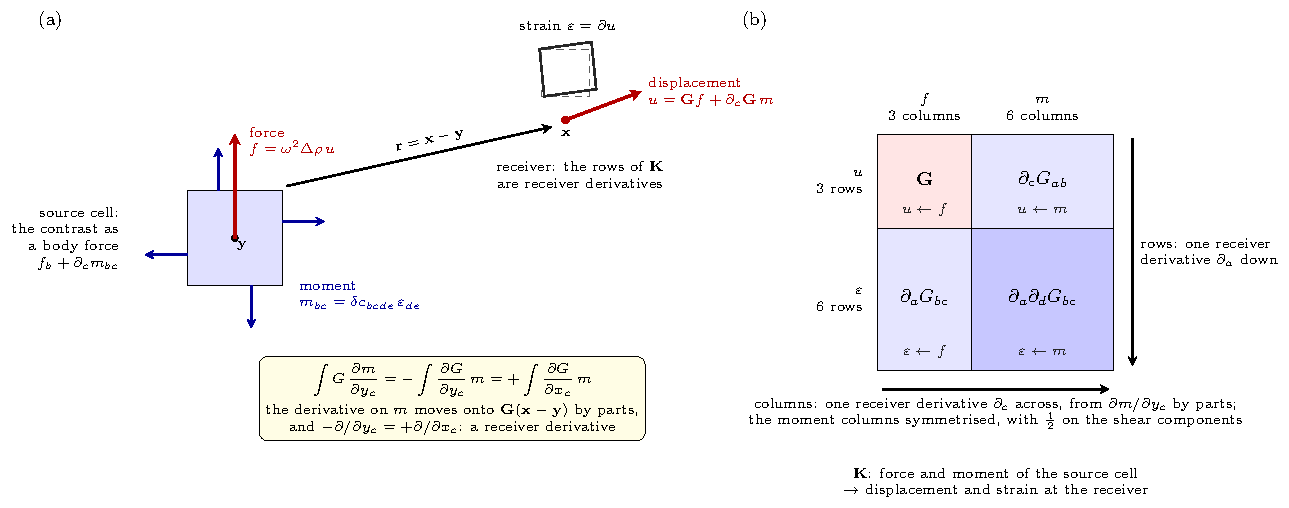
\includegraphics[width=\linewidth]{figures/fig_kernel.pdf}
\caption{Where the kernel comes from. (a) A source cell at $\mathbf y$ acts on the background through
the body force of Eq.~\eqref{eq:bodyforce}: a force $f$ from its density contrast, and the divergence
of its contrast stress $m$, the moment, from its stiffness contrast (arrows on the faces). At the
receiver $\mathbf x$ the state is the displacement $u$ and the strain $\varepsilon$. The moment's
derivative moves onto $\bG(\mathbf x-\mathbf y)$ by parts, Eq.~\eqref{eq:byparts}, and becomes a
receiver derivative with a plus sign. (b) The block structure of the $9\times9$ kernel $\bK$ that
results: the force columns are $\bG$, the moment columns carry one receiver derivative across, the
strain rows one receiver derivative down, and the strain-from-moment block two.}
\label{fig:kernel}
\par\smallskip{\footnotesize\textit{Alt text:} Two panels. On the left, a shaded square cell with a
dot at its centre marked y; a thick red arrow labelled force rises from the centre, and four blue
arrows labelled moment point outward from the cell's faces. A long arrow labelled r equals x minus y
runs from the cell to a red dot marked x at the upper right, from which a red arrow labelled
displacement leaves and above which a small dashed square deformed into a parallelogram is labelled
strain. A boxed line below reads: the integral of G times the y-derivative of m equals minus the
integral of the y-derivative of G times m, equals plus the integral of the x-derivative of G times m.
On the right, a two-by-two grid of shaded blocks with rows labelled u, three rows, and strain, six
rows, and columns labelled f, three columns, and m, six columns; the blocks read G, the first
derivative of G, the first derivative of G, and the second derivative of G; an arrow down the right
side reads rows: one receiver derivative down, and an arrow along the bottom reads columns: one
receiver derivative across.\par}
\end{figure}

\paragraph{Averaging, and collocation.} Three operations in this paper are averages over a cell,
and they are distinct. The \emph{source-cell average} integrates the kernel over the cell that
radiates: $\langle\bK\rangle(\mathbf r)=d^{-3}\int_{\text{cube}}\bK(\mathbf r-\mathbf y)\,\dd\mathbf y$
is the field at $\mathbf r$ of a uniform polarisation of the source cell. Every scheme in this paper
uses it, and it is exact for cubes that tile space \citep{NestorError2026}. \emph{Collocation} fixes where the discrete
equation is imposed: at the receiving cell's centre, with the internal field of each cell uniform, so
that the unknown is the field at the centre. The \emph{receiver-cell average} imposes the equation in
the mean over the receiving cell instead; with a uniform internal field that is the Galerkin scheme
of degree zero, called the mean-only voxel below. The two are both \emph{uniform-field} voxels, a
term that refers to the internal field and not to the test, and they differ only in the test
function (a delta at the centre against the cell's indicator) and in the constant of their
$O((kd)^2)$ error \citep{NestorError2026}. The \emph{cell-mean contrast}, finally, is an average of
the material, not of the field: where the medium varies within a cell, the contrast is projected
onto the cell's basis, its mean for degree $r=0$, rather than sampled at the centre
\citep{NestorError2026}. In the language of the coupled-dipole method, the point
dipole is collocation with the point kernel, the integrated Green tensor adds the source-cell
average, and the filtered coupled dipoles replace the point source by one of finite extent.

\paragraph{Implementations.} Every result is derived symbolically in Mathematica and compared with
an independent numerical implementation or an exact solution. ``The package'' below is the Python/Fortran
implementation of the voxel scheme (\path{cubic_scattering}): its cube $T$-matrix, its lattice
kernels and its stratified propagator, which serve both as the object under test and, where
validated, as a second implementation.


\section{The single site: the cube \texorpdfstring{$T$}{T}-matrix from moment integrals}\label{sec:single}

Every error of a voxel scheme is made at the single site \citep{NestorError2026}, so the single
site is derived here rather than imported. The classical route imports it. For an ellipsoid,
Eshelby's uniformity theorem makes the internal strain under a uniform load uniform, with a
depolarisation tensor in closed form \citep{Eshelby1957,Eshelby1959,Mura1987}; its dynamic
generalisation is known for spheres and ellipsoids \citep{FuMura1983,Mikata1990,Michelitsch2003}. For a
cube or a general polyhedron the static field of a uniform eigenstrain is also in closed form
\citep{Chiu1977,Rodin1996,Nozaki2001}, and it has been computed for a cuboid in an anisotropic matrix
\citep{LeeJohnson1978}, but the strain it produces is not uniform, so there is no exact uniform-strain
inclusion to import. Closed-form Eshelby tensors for polyhedral
inclusions with polynomial eigenstrains have since been given \citep{WuZhangYin2021}, the dynamic
inclusion problem has been formulated for shapes other than the ellipsoid, cubes among them
\citep{WangMichelitsch2005}, and the Green's tensor has been integrated analytically over a cuboid for
the coupled-dipole method, to an error of $O((kd)^4)$ \citep{YurkinSmunev2023}; these are the static
and electromagnetic counterparts of individual moments below. In scattering theory the volume integral
equation of an elastic inclusion \citep{Gubernatis1977} is closed in the same spirit by a
self-consistent or effective-field approximation \citep{MalKnopoff1967,Kanaun2008}: a first-order (Born) scatterer
\citep{Wu1985} renormalised by the geometric series of its own near field, the step that turns a
contrast into an effective contrast. \citet{Nestor1996} introduced the single site in this form,
summing the series of the cell's self integral, with the singular near field evaluated over an
infinitesimal cell. The moments below evaluate the same self integral over the finite cube, as a
distribution. The elastic $T$-matrix of \citet{Waterman1976} represents a
scatterer in spherical multipoles, the natural basis for a sphere; a voxel in a lattice needs one
compatible with the lattice, and the moments over the cube provide it. The construction below makes the
approximation of a voxel explicit rather than implicit: it derives the cube's $T$-matrix from
the moments of the elastodynamic Green's tensor over the cube, with the uniform-strain closure as the
first truncation of a hierarchy.

\paragraph{A Cartesian multipole hierarchy.} We call the construction the Cartesian multipole
hierarchy (Fig.~\ref{fig:multipole}). The contrast acting on the voxel's field is a source: the density
contrast a body force $\omega^2\Delta\rho\,\mathbf{u}$, the stiffness contrast a stress
$\delta\mathbf{c}:\boldsymbol\varepsilon$. Each voxel radiates through the Cartesian multipole moments of
these sources over the cube, a force monopole and a stress dipole from the uniform field (the cell of the
coupled-dipole method) and higher multipoles from the field's gradients, and receives the field through
its gradients at its centre. The name needs one caution. A multipole expansion usually expands the kernel
or the field about a centre and truncates it, which holds only for well-separated cells or outside a
circumscribing sphere: in the fast multipole method \citep{CarrierGreengardRokhlin1988}, whose
elastodynamic form leaves adjacent cells to direct integration \citep{ChaillatBonnetSemblat2007}, in the
spherical-wave $T$-matrix of \citet{Waterman1976}, and in the force-dipole description of a point defect,
an expansion of the Green's function far from it \citep{Clouet2018}. Here the Green's tensor is never
expanded. Only the source is resolved into Cartesian moments, and the integral over the source cube is
exact at every separation, so there is no radius of convergence, and touching voxels and the self term,
a distribution in closed form, are included. The source side is shared with the multipole extensions of
the coupled-dipole method in optics \citep{Evlyukhin2011,Ustimenko2022} and with Cartesian multipole
decompositions of a source \citep{Riccardi2022}. The word hierarchy has its sense in kinetic theory and
cosmology \citep{MaBertschinger1995}: a chain of coupled moment equations closed by truncation at a
chosen order, whose truncation error is here in closed form.

\paragraph{The multipole orders.} A hierarchy of degree $\ell$ holds the force density $\omega^2\Delta\rho\,
\mathbf{u}$ to degree $\ell$ and the stress $\delta\mathbf{c}:\boldsymbol\varepsilon$ to degree $\ell-1$.
A stress moment of degree $n$ acts on the medium through its divergence, as a force multipole of order
$n+1$, so both channels carry the force multipoles through order $\ell$ (Table~\ref{tab:multipoles}).
Here a multipole is the primitive Cartesian moment, which keeps its traces, rather than the irreducible
one \citep{Riccardi2022}. What sets the order of convergence is each channel's first omitted source
term, counted in its own degree (\S\ref{sec:blocks}): fourth order needs the force quadrupole for a
density contrast, but the second-degree stress moments, a force octupole, for a stiffness contrast.

\begin{table}[htbp]
\centering
\caption{The force multipoles a hierarchy of degree $\ell$ carries, and the order of convergence it
reaches for each contrast on the layer (Table~\ref{tab:hierlayer}).}\label{tab:multipoles}
\small
\begin{tabular}{@{}cllcc@{}}
\toprule
$\ell$ & density channel & stiffness channel & \multicolumn{2}{c}{order reached}\\
 & (force moments) & (stress moments) & density & stiffness\\
\midrule
$1$ & monopole, dipole & dipole & $2$ & $2$\\
$2$ & to the quadrupole & dipole, quadrupole & $4$ & $2$\\
$3$ & to the octupole & to the octupole & $4$ & $4$\\
\bottomrule
\end{tabular}
\end{table}

\begin{figure}[!htb]
\centering
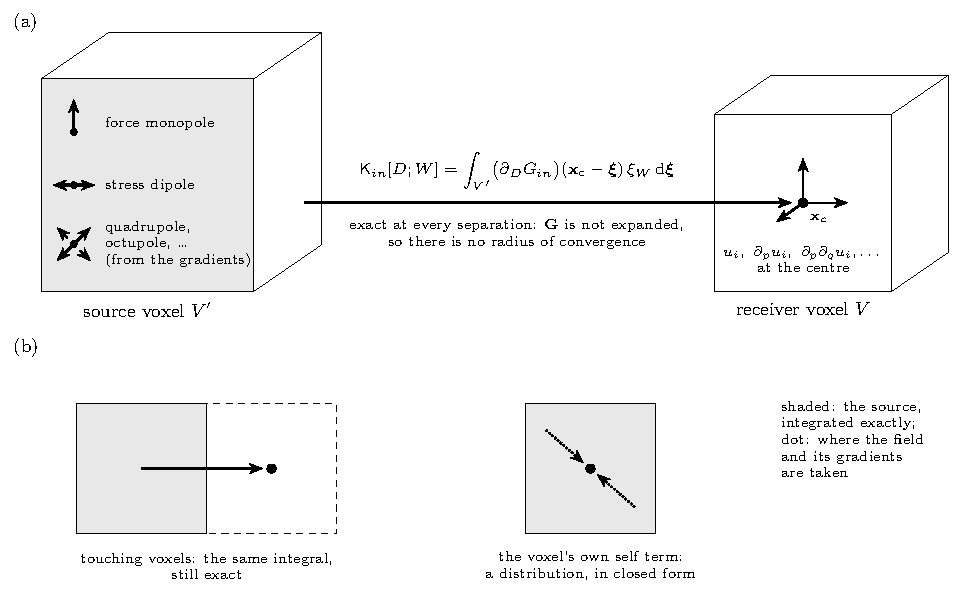
\includegraphics[width=\linewidth]{figures/fig_multipole.pdf}
\caption{The Cartesian multipole hierarchy. (a) The source voxel radiates through the Cartesian
multipole moments of its source: a force monopole from the density contrast, a stress dipole from the
stiffness contrast, and the quadrupoles, octupoles and higher multipoles from the field's
gradients. The receiver voxel takes the field
through its value and gradients at its centre $\mathbf x_c$. The two are coupled by the integral of the
derivatives of the Green's tensor over the whole source cube, Eq.~\eqref{eq:gradkernel}, which is exact
at every separation because the Green's tensor is not expanded. (b) The cases a multipole expansion of
the Green's tensor cannot reach are therefore included: touching voxels, by the same integral, and the
voxel's own self term, a distribution in closed form.}
\label{fig:multipole}
\par\smallskip{\footnotesize\textit{Alt text:} Two panels. In the upper panel a shaded cube on the left,
labelled source voxel, contains three small symbols: a single arrow labelled force monopole, a pair of
opposed arrows labelled stress dipole, and a cross of four arrows labelled quadrupole, octupole, and so on,
from the gradients. A long arrow runs from it to the centre of an unshaded cube on the right, labelled
receiver voxel, where a dot with three short arrows marks the field and its gradients at the centre.
Above the arrow is the coupling integral of the derivatives of the Green's tensor over the source cube,
and below it the words exact at every separation: G is not expanded, so there is no radius of
convergence. In the lower panel, on the left, a shaded square touches a dashed square whose centre is
marked by a dot, with an arrow from the shaded square to the dot, labelled touching voxels: the same
integral, still exact; on the right a single shaded square has a dot at its centre and two dotted arrows
pointing to it from within, labelled the voxel's own self term: a distribution, in closed form.}
\end{figure}

\paragraph{Its origin in the equivalent inclusion method.} In its static form the construction is the
equivalent inclusion method with polynomial eigenstrains of \citet{Moschovidis1975}: the eigenstrain
is expanded about the centre of the inhomogeneity, the consistency equation is expanded there in a
Taylor series, and the coefficient of each monomial is equated, which amounts to imposing the
Lippmann--Schwinger equation and its derivatives at the centre \citep[\S2.2]{Brisard2014}.
\citet{Johnson1980a,Johnson1980b} applied an expansion about the origin to a cuboidal
inhomogeneity, and \citet{WuZhangYin2021} expanded the eigenstrain of a polyhedron to second degree
about its centroid; both report that the expansion about the centre does not follow the field near the
edges, corners or vertices. \citet{FuMura1983} extended the method to time-harmonic waves for an
ellipsoid, with a second unknown for the density mismatch, and in the cases they report evaluated it
with uniform eigenstrains. \citet{Brisard2014} replaced the Taylor form by a Galerkin form of the same
equation, because the Taylor form need not give an invertible system and a higher degree need not
improve it. What is added here, to our knowledge, is the elastodynamic hierarchy, with density and
stiffness contrasts together, to any degree and for a body that is not an ellipsoid; its moments as
distributions in closed form; and the structure and the error of its truncations, tested degree by
degree against the exact solution for a sphere. The moments here are integrals of the Green's tensor
against monomials over the body. They are not moments in the sense of the method of moments
\citep{Harrington1993}, of which the hierarchy is the instance with monomials about the centre as
expansion functions and the $\delta$ function and its derivatives at the centre as testing functions;
and the exact static response of an inclusion of any shape to polynomial loads is described by the
polarisation and elastic moment tensors of \citet{AmmariKang2007}.

\subsection{The closed hierarchy}\label{sec:hierarchy}

Let the voxel be $V=[-h,h]^3$ with contrast
$\delta c_{ijkl}=\Delta\lambda\,\delta_{ij}\delta_{kl}+\Delta\mu(\delta_{ik}\delta_{jl}+\delta_{il}\delta_{jk})$
and $\Delta\rho$. The hierarchy is stated below for any degree; its third degree is written out
first, being the lowest at which the stiffness channel converges at fourth order (\S\ref{sec:blocks}).
Expand the internal displacement about the centre to third degree and project the
Lippmann--Schwinger equation onto $1$, $x_p$, $x_px_q$ and $x_px_qx_v$. The unknowns are $u_i(0)$,
$\partial_pu_i(0)$, $\partial_p\partial_qu_i(0)$ and $\partial_p\partial_q\partial_vu_i(0)$, and the
result is the closed system
\begin{align}
\bigl(\delta_{ij}-\omega^2\Delta\rho\,\mathsf G_{ij}\bigr)u_j
  +\bigl(\mathsf N^{r}_{in,k}\,\delta c_{nksj}-\tfrac12\omega^2\Delta\rho\,\mathsf K^{rs}_{ij}\bigr)
  \partial_r\partial_su_j
  &= u^0_i, \label{eq:A11}\\
\bigl(\delta_{pr}\delta_{ij}+\omega^2\Delta\rho\,\mathsf N^{r}_{ij,p}
  -\mathsf M_{in,pk}\,\delta c_{nkrj}\bigr)\partial_ru_j\qquad\qquad\qquad& \notag\\
  +\bigl(\tfrac16\omega^2\Delta\rho\,\mathsf B^{rst}_{ij,p}
  -\tfrac12\mathsf P^{st}_{in,pk}\,\delta c_{nkrj}\bigr)\partial_r\partial_s\partial_tu_j
  &= \partial_pu^0_i, \label{eq:A22}\\
-\omega^2\Delta\rho\,\mathsf M_{ij,pq}\,u_j
  +\bigl(\delta_{qr}\delta_{ps}\delta_{ij}+\mathsf Q^{r}_{in,pqk}\,\delta c_{nksj}
  -\tfrac12\omega^2\Delta\rho\,\mathsf P^{rs}_{ij,pq}\bigr)\partial_r\partial_su_j
  &= \partial_p\partial_qu^0_i, \label{eq:A33}\\
\bigl(\omega^2\Delta\rho\,\mathsf Q^{r}_{ij,pqv}-\mathsf X_{in,pqvk}\,\delta c_{nkrj}\bigr)\partial_ru_j
  \qquad\qquad\qquad\qquad& \notag\\
  +\bigl(\delta_{pr}\delta_{qs}\delta_{vt}\delta_{ij}+\tfrac16\omega^2\Delta\rho\,\mathsf J^{rst}_{ij,pqv}
  -\tfrac12\mathsf Z^{st}_{in,pqvk}\,\delta c_{nkrj}\bigr)\partial_r\partial_s\partial_tu_j
  &= \partial_p\partial_q\partial_vu^0_i, \label{eq:A44}
\end{align}
all fields evaluated at the centre. Dropping the third gradients, that is Eq.~\eqref{eq:A44} and the
second line of Eq.~\eqref{eq:A22}, leaves the system of second degree; dropping the second gradients
as well, that is Eq.~\eqref{eq:A33} and the $\partial\partial u$ terms of Eq.~\eqref{eq:A11}, leaves
the uniform-strain closure. Equations \eqref{eq:A11} and \eqref{eq:A33} are the same at second and
third degree, because every term the third degree would add to them vanishes by parity
(\S\ref{sec:parity}). The coefficients are ten moments of the background Green's tensor $\bG$ over
the voxel
\begin{equation}\label{eq:moments}
\begin{aligned}
\mathsf G_{ij}&=\int_V G_{ij}\,\dd V, &
\mathsf K^{rs}_{ij}&=\int_V G_{ij}\,x_rx_s\,\dd V, &
\mathsf N^{r}_{in,k}&=\int_V \partial'_kG_{in}\,x_r\,\dd V,\\
\mathsf M_{in,pk}&=\int_V \partial'_p\partial'_kG_{in}\,\dd V, &
\mathsf P^{rs}_{ij,pq}&=\int_V \partial'_q\partial'_pG_{ij}\,x_rx_s\,\dd V, &
\mathsf Q^{r}_{in,pqk}&=\int_V \partial'_q\partial'_p\partial'_kG_{in}\,x_r\,\dd V,\\
\mathsf B^{rst}_{ij,p}&=\int_V \partial'_pG_{ij}\,x_rx_sx_t\,\dd V, &
\mathsf J^{rst}_{ij,pqv}&=\int_V \partial'_v\partial'_q\partial'_pG_{ij}\,x_rx_sx_t\,\dd V, &
\mathsf X_{in,pqvk}&=\int_V \partial'_v\partial'_q\partial'_p\partial'_kG_{in}\,\dd V,\\
\mathsf Z^{rs}_{in,pqvk}&=\int_V \partial'_v\partial'_q\partial'_p\partial'_kG_{in}\,x_rx_s\,\dd V,
\end{aligned}
\end{equation}
the first six being those of the second degree and the last four those the third gradients add. The
derivatives are taken with respect to the source point, $\partial'=-\partial$. That sign reaches
the moments with an odd number of derivatives, $\mathsf N$, $\mathsf Q$, $\mathsf B$ and $\mathsf J$,
and no symmetry, parity or scaling check can detect it, so it is fixed by convention. The moments are
graded by $(D,W)$, the number of derivatives and the degree of the weight: $\mathsf G\,(0,0)$,
$\mathsf K\,(0,2)$, $\mathsf N\,(1,1)$, $\mathsf M\,(2,0)$, $\mathsf P\,(2,2)$, $\mathsf Q\,(3,1)$,
and $\mathsf B\,(1,3)$, $\mathsf J\,(3,3)$, $\mathsf X\,(4,0)$, $\mathsf Z\,(4,2)$.

\paragraph{The hierarchy at any degree.} Nothing in the construction is special to the third degree.
Let the internal displacement be expanded to degree $\ell$,
\begin{equation}\label{eq:taylorfield}
  u_j(\mathbf x)=\sum_{|W|\le\ell}\frac{x_W}{|W|!}\,U_{j;W},\qquad
  U_{j;W}=\partial_Wu_j(0),\quad x_W=x_{w_1}\cdots x_{w_m},
\end{equation}
the sum running over ordered sets of indices $W=(w_1,\dots,w_m)$, and let the strain be its derivative.
Write the moments with any number of derivatives and any weight as
\begin{equation}\label{eq:gmoment}
  \mathsf g_{in}[D;W]=\bigl\langle\partial_DG_{in},\ x_W\,\mathbf 1_V\bigr\rangle ,
\end{equation}
the derivatives being those of $G_{in}$ as a function of its argument and the pairing distributional
(\S\ref{sec:distributions}). The ten moments of Eq.~\eqref{eq:moments} are these $\mathsf g$
themselves: they are the integrals of $\partial'_D G_{in}(\mathbf 0-\mathbf x)$, and the factor
$(-1)^{|D|}$ of the source derivative cancels the parity $(-1)^{|D|}$ of $\partial_DG_{in}$, so that,
for example, $\mathsf N^r_{in,k}=\mathsf g_{in}[k;r]$ and $\mathsf Z^{rs}_{in,pqvk}=\mathsf
g_{in}[pqvk;rs]$. Beyond the third degree the moments are written as $\mathsf g$ only. Imposing the Lippmann--Schwinger
equation and its derivatives to order $\ell$ at the centre gives, for every set of derivative indices
$P$ with $|P|\le\ell$,
\begin{equation}\label{eq:hierarchy}
  U_{i;P}-(-1)^{|P|}\omega^2\Delta\rho\sum_{|W|\le\ell}\frac{\mathsf g_{ij}[P;W]}{|W|!}\,U_{j;W}
  +(-1)^{|P|}\sum_{|W|\le\ell-1}\frac{\mathsf g_{in}[Pk;W]}{|W|!}\,\delta c_{nkrj}\,U_{j;rW}
  =\partial_Pu^0_i(0).
\end{equation}
Equations \eqref{eq:A11}--\eqref{eq:A44} are the case $\ell=3$, with the moments of
Eq.~\eqref{eq:moments} put for the $\mathsf g$; their truncations above are $\ell=2$ and the
uniform-strain closure $\ell=1$. With the field rather than the eigenstrain as the unknown, the
moments $\mathsf g[D;W]$ play the part of the polynomial Eshelby tensors of the equivalent inclusion
method \citep[Ch.~4]{Mura1987}, which \citet{Brisard2014} call influence pseudotensors, here for the
elastodynamic kernel and for the density channel as well. For an ellipsoid the static self term of a
polynomial eigenstrain is itself a polynomial of the same degree, so the expansion about the centre is
exact in the self term and approximate only in the interaction with other bodies \citep{Brisard2014};
for a cube it is approximate in both. The cube is centrosymmetric, so a moment vanishes unless $|D|+|W|$ is even, and the system
needs the grades
\begin{equation}\label{eq:grades}
\begin{aligned}
  &(D,W)=(m,\,W),\quad W\le\ell &&\text{(density)},\\
  &(D,W)=(m+1,\,W),\quad W\le\ell-1 &&\text{(stiffness)},
\end{aligned}
  \qquad m=0,\dots,\ell,\quad D+W\ \text{even}.
\end{equation}
Table~\ref{tab:grades} lists what each degree adds. The unknowns number
$3\binom{\ell+3}{3}$: $12$, $30$, $60$ for $\ell=1$, $2$, $3$.
\begin{table}[htbp]
\centering
\caption{The grades $(D,W)$ of moments, $D$ derivatives on the Green's tensor and a weight of degree
$W$, that the hierarchy of degree $\ell$ needs beyond those of degree $\ell-1$.}\label{tab:grades}
\small
\begin{tabular}{@{}cll@{}}
\toprule
$\ell$ & new grades & moments in all \\
\midrule
$1$ & $(0,0)$, $(1,1)$, $(2,0)$ & $3$ \\
$2$ & $(0,2)$, $(2,2)$, $(3,1)$ & $6$: $\mathsf G$, $\mathsf K$, $\mathsf N$, $\mathsf M$, $\mathsf P$, $\mathsf Q$ \\
$3$ & $(1,3)$, $(3,3)$, $(4,0)$, $(4,2)$ & $10$: with $\mathsf B$, $\mathsf J$, $\mathsf X$, $\mathsf Z$ \\
$4$ & $(0,4)$, $(2,4)$, $(4,4)$, $(5,1)$, $(5,3)$ & $15$ \\
$5$ & $(1,5)$, $(3,5)$, $(5,5)$, $(6,0)$, $(6,2)$, $(6,4)$ & $21$ \\
\bottomrule
\end{tabular}
\end{table}

\paragraph{Two independent systems.} In either sum of Eq.~\eqref{eq:hierarchy} the unknown
$U_{i;P}$ is coupled to $U_{j;W}$, or to $U_{j;rW}$, through a moment of grade $(|P|,|W|)$ or
$(|P|+1,|W|)$, and on a centrosymmetric body that moment vanishes unless $|P|$ and the degree of the
unknown it multiplies have the same parity. The hierarchy of any degree therefore separates exactly,
at every frequency and contrast, into two systems: one for the even gradients $u$,
$\partial\partial u,\dots$ and one for the odd gradients $\partial u$, $\partial\partial\partial
u,\dots$. Raising the degree from odd to even adds a block to the even system alone, and from even to
odd a block to the odd system alone. At $\ell=3$ the even system is Eqs.~\eqref{eq:A11} and
\eqref{eq:A33}, unchanged from $\ell=2$, and the odd system is Eqs.~\eqref{eq:A22} and \eqref{eq:A44}.
Of the sixty unknowns, twenty-one belong to the even system and thirty-nine to the odd. The leading radiation of a density contrast,
$\int_V\Delta\rho\,u\,\dd V$, is drawn from the even system, and that of a stiffness contrast,
$\int_V\delta c:\nabla u\,\dd V$, from the odd one. The separation is thus the structure behind the
result of \S\ref{sec:blocks}, that the blocks improve the density and the stiffness channels
alternately. At first degree it is implicit in the dynamic equivalent inclusion method for an
ellipsoid, where the force and the strain systems uncouple at the centre \citep{FuMura1983}; here it
holds at every degree, for any centrosymmetric body.

\subsection{The moments as distributions}\label{sec:distributions}

Write the elastodynamic tensor as
\begin{equation}\label{eq:Gdecomp}
  G_{in}(\mathbf r)=\frac{1}{4\pi\mu}\Bigl[\delta_{in}\,g_{S}(r)
  +\frac{1}{k_S^2}\,\partial_i\partial_n\bigl(g_S(r)-g_P(r)\bigr)\Bigr],
  \qquad g_{c}(r)=\frac{\mathrm{e}^{\mathrm{i}k_cr}}{r}
\end{equation}
\citep{Kupradze1963,Aki2002}. Expanding $g_c$ in powers of $r$ reduces every moment in
Eq.~\eqref{eq:moments} to a finite sum of scalar moments
\begin{equation}\label{eq:Emoment}
  E\bigl[m;d_1\ldots d_D;w_1\ldots w_W\bigr]
  =\bigl\langle \partial_{d_1}\!\cdots\partial_{d_D}\,r^m,\ x_{w_1}\!\cdots x_{w_W}\,\mathbf 1_V\bigr\rangle .
\end{equation}
For $m=-1$ and $D\ge2$ the classical integrand is not absolutely integrable. $\partial^2(1/r)$
decays as $r^{-3}$, its angular average vanishes, and the value of the integral depends on the
shape of the region excluded around the origin. This is the source of the $\delta$-function term
of the inclusion problem, which a numerical quadrature misses. Without it the depolarisation is
wrong; for a sphere it vanishes altogether (\S\ref{sec:parity}). It is not added afterwards here. The derivatives are
distributional from the start, and each is moved onto the voxel's faces by pairing with the test
function $w\mathbf 1_V$, using $\partial_q\mathbf 1_V=-n_q\,\delta_{\partial V}$:
\begin{equation}\label{eq:peel}
  \bigl\langle \partial_qT,\,w\mathbf 1_V\bigr\rangle
  =\oint_{\partial V} n_q\,w\,T\,\dd A-\bigl\langle T,\,(\partial_qw)\,\mathbf 1_V\bigr\rangle .
\end{equation}
The surface term is evaluated on the faces, a distance $h$ from the origin, where every
derivative of $r^m$ is smooth. The recursion lowers $D$ and $W$ together and ends on convergent
integrals. The face integrals are done in closed form by the corner sums of the tiling identity \citep{NestorError2026}. The
sharp check is the sum rule
\begin{equation}\label{eq:sumrule}
  \textstyle\sum_pE[-1;p,p;\,]=\nabla^2(1/r)\ \text{paired with}\ \mathbf 1_V=-4\pi ,
\end{equation}
which the face route satisfies exactly and a spherical excision returns as $0$. The closed forms
contain logarithms of the units $(2\pm\sqrt3)^n$ of the Pell equation $x^2-3y^2=1$. Left
unreduced, these cancel catastrophically: for example, $\log(72010600134783751-41575339372323900\sqrt3)$
is a cancellation of $35$ digits. They are therefore reduced to $n\log(2-\sqrt3)$, which is
exact. Because every power of $r$ is paired this way, the dynamic moments keep the even-power terms
of the expansion ($k^2r$, $r^3$, \dots) as well as the odd ones. A route that integrates only the
polynomial (odd-power) terms of $\bG$ misses those terms, at a real $O((kh)^2)$ cost
(\S\ref{sec:closure}).

\paragraph{Every grade, in closed form on four constants.} Closed forms for monomial-weighted
integrals of $1/r$ over bricks are known \citep{Hackbusch2002}, as are closed forms for the potential
and its first two derivatives over polyhedra with polynomial density, from the gravity literature
\citep{Ren2020}. The engine used here differs in taking derivatives of any order as distributions, in
treating the kernel $r$ as well as $1/r$, and in the even-power terms of the dynamic series. The
recursion \eqref{eq:peel} does not
depend on the grade, so the same engine gives every scalar moment of Table~\ref{tab:grades}. Each is
evaluated once and stored. The scalar moments of every grade through $\ell=5$, with up to six
derivatives and weights to the fifth degree, have been evaluated for the kernels $r^{-1}$ and $r$:
$4224$ closed forms. (The second term of Eq.~\eqref{eq:Gdecomp} places two further derivatives on
$r$; those moments are stored through $\ell=3$ and are evaluated numerically, by the second route
below, beyond it.) Every one of them is a power of the voxel's width times
\begin{equation}\label{eq:fourconstants}
  q_0+q_1\sqrt3+q_2\,\pi+q_3\log\bigl(2-\sqrt3\bigr),\qquad q_i\ \text{rational}.
\end{equation}
The integration returns many of them in other forms, with $\log(\sqrt3-1)$, $\log(1+\sqrt3)$, inverse
hyperbolic tangents and logarithms of powers of two, which are equal in value but not canonical: two
equal moments can then differ in appearance, and sums of large logarithms that cancel lose digits. Each
stored form is therefore reduced to Eq.~\eqref{eq:fourconstants} by an integer-relation search at $400$
digits, with $\log2$ and $\log3$ admitted to the search, and the reduction is accepted only if it agrees
with the stored form to $1200$ digits. All $4224$ reduce, and the coefficients of $\log2$ and $\log3$
are zero in every one.

Every grade is gated by two checks whose answers do not depend on the engine, the Laplacian
sum rules of Eq.~\eqref{eq:gates}, which test the $\delta$ function of the inclusion problem and its
derivatives where a quadrature fails, and confirmed by a second route that shares nothing with the
faces of the cube, to $1.1\times10^{-12}$ or better (Appendix~\ref{app:engine}).

\subsection{Parity, and the nine-component block}\label{sec:parity}

The cube is centrosymmetric. A moment that couples a field quantity of degree $a$ to one of degree
$b$ therefore vanishes unless $a+b$ is even. $u$, $\partial u$ and $\partial\partial u$ have
degrees $0$, $1$ and $2$, so at second degree Eq.~\eqref{eq:A22} contains the first gradient alone:
$\partial u$ is determined by its own block and couples to neither $u$ nor $\partial\partial u$. At
any degree it couples to nothing of even degree; from $\ell=3$ it couples to $\partial\partial\partial u$
(the second line of Eq.~\eqref{eq:A22}). The leading
scattering by a stiffness contrast is the stress dipole $\int_V\delta c:\nabla u\,\dd V$, which needs
only $\partial u$. The leading far field of the stiffness contrast is therefore fixed by
Eq.~\eqref{eq:A22}, and \emph{no treatment of the second-gradient block \eqref{eq:A33} can change
it}. What Eq.~\eqref{eq:A33} contributes reaches the far field only through the $O((kh)^2)$
coupling in Eq.~\eqref{eq:A11}. That is the order, and the origin (the variation of the field
across the voxel), of the collocation error on the layer, which the first-moment
voxel removes \citep{NestorError2026}, as does the hierarchy itself once its third-gradient block is kept
(\S\ref{sec:blocks}).

\paragraph{The symmetry of the cube.} The cube is unchanged by $48$ operations: the $24$ rotations
that carry it into itself, each with or without the inversion $\mathbf x\to-\mathbf x$. They form the
group $O_h$. Any operator built from the cube alone commutes with all $48$, and group theory then says
how far it can be simplified \citep{Tinkham1964,Dresselhaus2008}. The quantities it acts on split into
irreducible representations, the smallest sets of components that the symmetry operations mix only among
themselves. Such an operator has no matrix elements between different representations, and on a
representation that occurs once it is a multiple of the identity (Schur's lemma). It is then diagonal,
with one eigenvalue for each representation, however many components that representation has. The
labels are the standard ones of crystal physics. $A$, $E$ and $T$ are representations of dimension one,
two and three, and the subscript $g$ (from the German \emph{gerade}, even) marks those that are even under
inversion, as a strain is. For the nine components of a displacement gradient, $A_{1g}$ is the dilatation,
$E_g$ the two traceless combinations of the diagonal strains, $T_{2g}$ the three off-diagonal shears, and
$T_{1g}$ the three rotations, the antisymmetric part of the gradient. A stiffness contrast acts on strain
only, so on $T_{1g}$ the operator below is the identity. A sphere is invariant under every rotation, not
only the cube's, and there $E_g$ and $T_{2g}$ join into a single five-dimensional shear channel. The cube
splits that channel into two and three dimensions, which is why its two shear eigenvalues are averaged
with the weights $2$ and $3$ in Eq.~\eqref{eq:shearsplit} below.

With $\Delta\rho=0$, Eq.~\eqref{eq:A22} at second degree is the $9\times9$ operator
$\delta_{pr}\delta_{ij}-\mathsf M_{in,pk}\,\delta c_{nkrj}$, built from $\mathsf M$ alone. Under
$O_h$ the nine gradient components decompose as $A_{1g}\oplus E_g\oplus T_{1g}\oplus T_{2g}$, and
the operator is diagonal in that basis. Its eigenvalues are the inverse strain concentrations:
\begin{align}
A_{1g}\ \text{(dilatation)}:&\quad 1+\frac{\Delta\lambda+\tfrac23\Delta\mu}{\lambda+2\mu},
  \label{eq:A1g}\\
T_{2g}\ \text{(off-diagonal shear)}:&\quad 1+2\Delta\mu\,S_{\text{off}},\qquad
  S_{\text{off}}=\frac{\pi(\lambda+2\mu)-\sqrt3\,(\lambda+\mu)}{3\pi\mu(\lambda+2\mu)},
  \label{eq:T2g}\\
E_{g}\ \text{(diagonal shear)}:&\quad 1+2\Delta\mu\,S_{\text{diag}},\qquad
  S_{\text{diag}}=\frac{3\sqrt3\,(\lambda+\mu)+2\pi\mu}{6\pi\mu(\lambda+2\mu)}.
  \label{eq:Eg}
\end{align}
The density channel is the displacement block of Eq.~\eqref{eq:A11} with the second gradients
dropped, an amplification $(1-\omega^2\Delta\rho\,\mathsf G)^{-1}$ with $\mathsf G$ the cube
integral of $\bG$.

\paragraph{The cube against the sphere.} For a sphere, Eshelby's tensor gives a dilatational
channel $1+\Delta K/(\lambda+2\mu)$, with $\Delta K=\Delta\lambda+\tfrac23\Delta\mu$, and a single
deviatoric channel $1+2\Delta\mu\,S_{\text{sph}}$, with $2\mu S_{\text{sph}}=2(4-5\nu)/[15(1-\nu)]$.
The cube's dilatational channel, Eq.~\eqref{eq:A1g}, is the sphere's exactly: its eigenvalue
involves $\mathsf M$ only through the contraction $\int_V\partial_i\partial_nG_{in}\,\dd V$, and the
static Navier equation makes $\partial_i\partial_nG_{in}=-\delta(\mathbf r)/(\lambda+2\mu)$, whose
integral does not depend on the shape. The
cube's shear channels differ from each other. Their isotropic average, however, is the sphere's,
also exactly:
\begin{equation}\label{eq:shearsplit}
  \tfrac15\bigl(3S_{\text{off}}+2S_{\text{diag}}\bigr)=S_{\text{sph}},\qquad
  S_{\text{diag}}-S_{\text{off}}=\frac{(\lambda+\mu)(5\sqrt3-2\pi)}{6\pi\mu(\lambda+2\mu)}>0 .
\end{equation}
The $\sqrt3$ terms cancel in the average. What a cube adds to a sphere at this order is therefore
a pure cubic anisotropy. It splits the deviatoric channel about the sphere's value, weighted $3:2$
by the dimensions of $T_{2g}$ and $E_g$, and the diagonal shear is the more depolarised. At the background of the tests
($\alpha=5000$, $\beta=3000$\,m\,s$^{-1}$, $\nu=7/32$), $2\mu S_{\text{off}}=0.4314$, $2\mu S_{\text{diag}}=0.5929$
and the sphere's value is $0.4960$.

\paragraph{Where Eshelby enters.} Equations \eqref{eq:A1g}--\eqref{eq:Eg} follow from the moment
integrals and the group theory alone. No ellipsoidal result is used, and no $\delta$ term is added
by hand. What corresponds to Eshelby is the \emph{truncation}. Keeping $\partial u$ and discarding
$\partial\partial u$ is exactly the uniform-internal-strain ansatz, and by the uniformity theorem
that ansatz is exact if and only if the inclusion is an ellipsoid. For a sphere the construction
is therefore exact in the static limit, and for a cube it is an approximation. The hierarchy
\eqref{eq:hierarchy} states that approximation as the omitted blocks, rather than as an
unquantified shape correction. A polynomial expansion about the centre cannot represent the edge
and corner concentrations of an isolated cube's internal field at any finite degree;
Table~\ref{tab:hiercube} measures what each degree leaves. A voxel in a
uniform layer has no such concentrations: its neighbours have the same properties, so its internal
field is the continuum's, which is smooth. That is why a low-degree internal field suffices in a
lattice \citep{NestorError2026} although it is only an approximation for an
isolated cube.

\paragraph{Against the exact sphere.} These statements are tested against the exact elastic Mie
solution, with no Eshelby formula in between (Appendix~\ref{app:closuremie}). Applied to a ball, the
construction's dilatational and shear channels equal Mie's static concentrations to $2\times10^{-10}$,
and the cube's dilatational channel and isotropic shear average meet the same numbers; taken as a
principal value the moment has no depolarisation at all, so the whole static response is the
$\delta$ term. At finite frequency the closure departs from Mie only by a real term of order $(ka)^2$
at first order in the contrast, given in closed form in Eq.~\eqref{eq:spheredynamic}; the radiation
damping is exact. That term is the uniform-field ansatz's own error, the order the hierarchy assigns
to the omitted second gradients.

\subsection{What each block of the hierarchy buys}\label{sec:blocks}

A hierarchy invites the question of what its next block is worth. The answer has a simple form, and it
is not the one a count of unknowns suggests: the blocks help in pairs.

\paragraph{The experiment.} The layer of \citet{NestorError2026} ($D=2$\,m, $\Delta\lambda=2$\,GPa, $\Delta\mu=1$\,GPa,
$\Delta\rho=100$\,kg\,m$^{-3}$ in the background above, $\rho=2500$\,kg\,m$^{-3}$) at normal incidence is cut into $n$
cells, and in each the hierarchy of degree $\ell$ is imposed: the displacement is its Taylor polynomial
of degree $\ell$ about the centre, the strain the derivative of that, and the equation and its first
$\ell$ derivatives hold at the centre, with the $\delta$ terms kept. In one dimension the moments are
elementary and the exact layer is known, so the order of each truncation can be measured for a density
contrast, a modulus contrast and both. The schemes are computed symbolically to $60$ digits for $\ell=1$ to $6$
and, to $\ell=3$, independently in double precision.

\paragraph{The prediction.} A cell radiates the integral of its source against the kernel. If the
source is held to a polynomial of degree $d$ about the centre, the first power it omits is $d+1$. When
$d+1$ is odd, that term integrates to zero against the even part of the kernel and the error is two
orders smaller; when $d+1$ is even it does not. The density source is the displacement, of degree
$\ell$; the stiffness source is the strain, of degree $\ell-1$. So a density contrast gains an order
pair at every even $\ell$, and a stiffness contrast at every odd $\ell$. This is the parity of
\S\ref{sec:parity}, read as an order of convergence.

\begin{table}[htbp]
\centering
\caption{The order of convergence of the hierarchy of degree $\ell$ on the layer, measured from $16$ to
$32$ cells in reflection and in transmission at $\omega=300$\,rad\,s$^{-1}$, and its reflection error on
$16$ cells with both contrasts. Every measured order equals the predicted one to the digits
shown.}\label{tab:hierlayer}
\small
\begin{tabular}{@{}lcccccc@{}}
\toprule
 & $\ell=1$ & $2$ & $3$ & $4$ & $5$ & $6$ \\
\midrule
density contrast only & $2$ & $4$ & $4$ & $6$ & $6$ & $8$ \\
modulus contrast only & $2$ & $2$ & $4$ & $4$ & $6$ & $6$ \\
both & $2$ & $2$ & $4$ & $4$ & $6$ & $6$ \\
error, both, $n=16$ & $5.4\times10^{-6}$ & $1.4\times10^{-6}$ & $5.8\times10^{-12}$ & $9.5\times10^{-13}$
  & $2.6\times10^{-18}$ & $3.1\times10^{-19}$ \\
\bottomrule
\end{tabular}
\end{table}

\paragraph{The result.} Table~\ref{tab:hierlayer}: all thirty-six orders are as predicted. The second
gradients raise the density channel to fourth order and leave the stiffness channel at second, with a
constant three to four times smaller in reflection; the third gradients bring the stiffness channel to fourth
order; and so on in pairs. With both contrasts, fourth order therefore needs $\ell=3$ and sixth order
$\ell=5$. The truncation of Eqs.~\eqref{eq:A11}--\eqref{eq:A44} at second gradients is one block short
of the next order for a stiffness contrast, which is why it improves the uniform-strain closure by a
constant and not by an order.

\paragraph{The error in closed form.} At first order in the contrast a cell whose source is held to
its Taylor polynomial of degree $d$ returns the exact term times $1+E_d$, where, with $h$ the
half-width,
\begin{equation}\label{eq:taylorfactor}
  E_d=\begin{cases}
  (-1)^{(d-1)/2}\,\dfrac{(kh)^{d+1}}{(d+2)!} & d\ \text{odd},\ R\ \text{and}\ T,\\[10pt]
  (-1)^{d/2}\,\dfrac{(kh)^{d+2}}{(d+2)!} & d\ \text{even},\ R,\\[10pt]
  (-1)^{d/2+1}\,\dfrac{(d+1)\,(kh)^{d+2}}{(d+3)!} & d\ \text{even},\ T,
  \end{cases}
\end{equation}
$R$ and $T$ standing for reflection and transmission,
with $d=\ell$ for the density term and $d=\ell-1$ for the stiffness term. It follows from the series of
$\int_{-1}^{1}P_d(\mathrm{i}khx)\,\mathrm{e}^{\mp\mathrm{i}khx}\,\dd x$ with $P_d$ the Taylor polynomial
of $\mathrm{e}^{\mathrm{i}khx}$, and it is confirmed symbolically for $d=0$ to $6$ and against the
scheme on one cell, at a contrast of $10^{-20}$ and $kh=0.03$, to $0.5\%$ in all twelve cases. For
$d=0$ it is $(kd)^2/8$ in reflection and $-(kd)^2/24$ in transmission: the constants of the collocation
scheme \citep{NestorError2026}, which are thus the first rung of a ladder
(\nb{ContinuumLimit\_GradientHierarchy.wl}, \path{scripts/measure_layer_taylor_hierarchy.py}).

\subsection{The single site against a sphere and a cube}\label{sec:singlesite}

The hierarchy is a statement about one scatterer, so it is tested first on one scatterer. The assembly
of Eq.~\eqref{eq:hierarchy}, with the full tensor moments in their dynamic form (the series of
$\mathrm{e}^{\mathrm{i}kr}/r$ taken to $r^{11}$), is the same for any centrosymmetric body; only the
scalar moments change.

\paragraph{A sphere.} For a ball the scalar moments are elementary, by the surface route of
Eq.~\eqref{eq:peel} on $|\mathbf r|=a$, and the exact answer is known. A homogeneous sphere of radius
$a=10$\,m with the contrast of the layer is illuminated by a P plane wave; the hierarchy's
polynomial source is radiated to nine scattering angles between $11^\circ$ and $169^\circ$, and the
error is the largest component of the difference from the exact displacement
\citep{YingTruell1956,PaoMow1973} over the largest exact component. The prediction, from the pairs of
\S\ref{sec:blocks} with $kh$ replaced by $ka$, is an error of $O((ka)^2)$ for $\ell=1$ and $2$ and of
$O((ka)^4)$ for $\ell=3$, and $O((ka)^4)$ already at $\ell=2$ for a density contrast alone.
\begin{table}[htbp]
\centering
\caption{One homogeneous sphere by the hierarchy of degree $\ell$: relative far-field error against
exact scattering, and the order between the two lowest frequencies. All nine orders are as
predicted.}\label{tab:hiersphere}
\small
\begin{tabular}{@{}llccccc@{}}
\toprule
contrast & $\ell$ (unknowns) & $k_Sa=0.4$ & $0.2$ & $0.1$ & order & predicted \\
\midrule
density only & $1$ ($12$) & $6.4\times10^{-3}$ & $1.6\times10^{-3}$ & $3.9\times10^{-4}$ & $2.0$ & $2$ \\
 & $2$ ($30$) & $4.8\times10^{-5}$ & $2.6\times10^{-6}$ & $1.8\times10^{-7}$ & $3.9$ & $4$ \\
 & $3$ ($60$) & $1.5\times10^{-5}$ & $9.5\times10^{-7}$ & $6.9\times10^{-8}$ & $3.8$ & $4$ \\
moduli only & $1$ & $1.9\times10^{-2}$ & $5.0\times10^{-3}$ & $1.1\times10^{-3}$ & $2.3$ & $2$ \\
 & $2$ & $5.4\times10^{-3}$ & $1.4\times10^{-3}$ & $3.4\times10^{-4}$ & $2.0$ & $2$ \\
 & $3$ & $6.2\times10^{-5}$ & $4.1\times10^{-6}$ & $2.0\times10^{-7}$ & $4.3$ & $4$ \\
both & $1$ & $1.4\times10^{-2}$ & $3.1\times10^{-3}$ & $7.2\times10^{-4}$ & $2.1$ & $2$ \\
 & $2$ & $3.2\times10^{-3}$ & $6.9\times10^{-4}$ & $1.8\times10^{-4}$ & $1.9$ & $2$ \\
 & $3$ & $4.6\times10^{-5}$ & $2.5\times10^{-6}$ & $1.4\times10^{-7}$ & $4.2$ & $4$ \\
\bottomrule
\end{tabular}
\end{table}
Table~\ref{tab:hiersphere} bears the prediction out. At $k_Sa=0.4$ the error of the uniform-strain
closure is $1.4\%$, that of the second-gradient system $0.32\%$, and that of the third-gradient system
$0.0046\%$: three hundred times below the closure. The systems are well conditioned, the sixty
equations of $\ell=3$ having a condition number of $5.9$
(\path{scripts/measure_ball_gradient_hierarchy.py}).

\paragraph{A cube.} The same assembly with the cube's moments gives the single site of a voxel. No
exact solution exists for a cube, so the reference is the same cube, of half-width $h=10$\,m, solved by
the Legendre voxels of \citet{NestorError2026} on refined grids, a cube being the one body such a grid
represents exactly. Solutions with first and second moments on $2^3$ and $3^3$ cells differ among
themselves by at most $2\times10^{-5}$, which is the accuracy of the reference.
\begin{table}[htbp]
\centering
\caption{One homogeneous cube of half-width $h$ by the hierarchy of degree $\ell$: relative far-field
error against the converged reference.}\label{tab:hiercube}
\small
\begin{tabular}{@{}lcccc@{}}
\toprule
$\ell$ (unknowns) & $k_Sh=0.4$ & $0.2$ & $0.1$ & $0.05$ \\
\midrule
$1$ ($12$) & $2.1\times10^{-2}$ & $5.4\times10^{-3}$ & $2.8\times10^{-3}$ & $2.7\times10^{-3}$ \\
$2$ ($30$) & $3.2\times10^{-3}$ & $1.6\times10^{-3}$ & $1.9\times10^{-3}$ & $2.4\times10^{-3}$ \\
$3$ ($60$) & $3.5\times10^{-4}$ & $3.4\times10^{-4}$ & $2.9\times10^{-4}$ & $3.1\times10^{-4}$ \\
\bottomrule
\end{tabular}
\end{table}
Table~\ref{tab:hiercube} shows what distinguishes a cube from a sphere. Each truncation has a floor that
does not fall with the frequency, because the internal field of an isolated cube is not a polynomial
even statically: it concentrates at the edges and corners, as the static expansions about the centre
of \citet{Johnson1980b} and \citet{WuZhangYin2021} found for the cuboid and for polyhedra. The floor is $2.7\times10^{-3}$ for the
uniform-strain closure and nearly the same with second gradients, as \S\ref{sec:parity} requires, the
static stress dipole being fixed by the first-gradient block and coupled next to the third. The
third-gradient block lowers it ninefold, to $3\times10^{-4}$. Above the floor the error falls with the
frequency as on the sphere: at $k_Sh=0.4$ the third-gradient system is sixty times more accurate than
the closure. The dip of the second-gradient row at $k_Sh=0.2$ is a cancellation between its static and
dynamic terms, which have opposite signs. The condition numbers lie between $11$ and $13$
(\path{scripts/measure_cube_gradient_hierarchy.py}). These results come from one implementation,
checked against the exact sphere and against the converged cube; the moments it uses are those
confirmed by two routes in \S\ref{sec:distributions}.

\subsection{The collocation closure}\label{sec:closure}

The collocation closure takes the internal field of a voxel as uniform, the truncation of
\S\ref{sec:parity} for the density and stiffness channels together. The voxel's own field at its
centre is then $\bS_{\text{self}}\bD\,e$ for internal state $e$, where $\bS_{\text{self}}$ is the
nine-component form of the moments $\mathsf G$ and $\mathsf M$. By parity it is block-diagonal. So
$e=\psi+\bS_{\text{self}}\bD e$ and
\begin{equation}\label{eq:closure}
  \bT=d^3\,\bD\bigl(\bI-\bS_{\text{self}}\bD\bigr)^{-1}.
\end{equation}
With the source-averaged kernel of a lattice of cubes the self term cancels, and the discrete system
becomes the collocation of the continuum Lippmann--Schwinger equation with a strain piecewise constant
over voxels: every block of its kernel is an exact cell integral, and $\bS_{\text{self}}$ does not appear
\citep{NestorError2026}.

The package's cube $T$-matrix is this closure statically: both blocks agree with
Eq.~\eqref{eq:closure} to $2\times10^{-5}$ at $k_Sh=0.01$, the difference falling
as $(kh)^2$ (\nb{ContinuumLimit\_CubeT.wl}). It departs dynamically by about $0.25(kh)^2$ through its
far-field form-factor corrections. Its self integrals are exact in the static and radiation parts
but omit the real even-power terms of the Green's tensor's expansion ($k^2r$, $r^3$, \dots), an
error of $0.4$--$0.6\,(kh)^2$ against the analytic self term, whose series agrees with the
closed-form elastodynamic tensor to $10^{-14}$. Since the self term does not appear in the collocation scheme, that error cannot enter
the closure scheme.

\subsection{What a closed-form single-site $T$-matrix gives}\label{sec:whyclosed}

The Cartesian multipole hierarchy costs more to set up than the alternatives: moments of the Green's
tensor to fourth derivatives, evaluated as distributions and reduced to closed form. What that buys
follows from the Lippmann--Schwinger equation of one body rather than from a model fitted to it.
\emph{One derivation.} The static depolarisation, its dynamic corrections, the radiation damping and
every higher block come from that one equation and one engine (\S\ref{sec:distributions}), so they
cannot be inconsistent with one another, and the static, spherical and low-frequency limits are results
of the construction rather than conditions imposed on it. \emph{Nothing is fitted.} Every coefficient of
Eq.~\eqref{eq:hierarchy} is a moment of the background Green's tensor over the body: there is no
polarisability to choose and no depolarisation factor to calibrate, where other routes import the single
site from the ellipsoid \citep{Eshelby1957,Mura1987} or close the volume integral equation with an
effective field \citep{MalKnopoff1967,Kanaun2008}. As in the equivalent inclusion method
\citep{Moschovidis1975,FuMura1983}, the uniform-strain closure is the first member (\S\ref{sec:parity});
what the hierarchy adds is the closed form at finite frequency for a body that is not an ellipsoid, with
the error of each truncation known. \emph{The singular self-interaction is exact}: the $\delta$-function
content that a quadrature misses is part of the moments from the start, and the sum
rule~\eqref{eq:sumrule} and the traces~\eqref{eq:gates} hold at every grade (\S\ref{sec:distributions}).
\emph{The exact limits are built in}: the cube's dilatational channel and its isotropic shear average
equal the sphere's, confirmed against the exact Mie solution to $2\times10^{-10}$ and $10^{-8}$
(\S\ref{sec:parity}), and at finite frequency the closure departs from Mie only through a real term of
order $(ka)^2$, the radiation damping agreeing exactly in all three channels
(Eq.~\eqref{eq:spheredynamic}). \emph{The error is stated before anything is solved}: a truncation is a
statement of which blocks are omitted; the orders come in the predicted parity pairs, all thirty-six on
the layer and all nine on the sphere (Tables~\ref{tab:hierlayer} and~\ref{tab:hiersphere}), and the
leading error factor is in closed form, Eq.~\eqref{eq:taylorfactor}. \emph{It improves block by block,
on fixed constants}: raising the degree adds moments, confirmed by a second route that shares nothing
with the first (\S\ref{sec:distributions}), and no quadrature; against the exact sphere at $k_Sa=0.4$
the error falls from $1.4\%$ for the uniform-strain closure to $0.0046\%$ with third gradients, from a
system of sixty equations with a condition number of $5.9$ (Table~\ref{tab:hiersphere}). That each degree
improves on the one below is shown here for one sphere and one cube, not in general: in the Taylor form
of the equivalent inclusion method, for interacting inhomogeneities, a higher degree need not improve
the solution and the system need not be invertible \citep{RodinHwang1991,Brisard2014}. \emph{It says
what a body's shape does}: at the order of the uniform-strain closure a cube is a sphere plus a pure
cubic anisotropy, which splits the deviatoric channel about the sphere's value in the ratio $3:2$
(Eq.~\eqref{eq:shearsplit}). \emph{It describes a scatterer, not only a cell}: the assembly is the same
for every centrosymmetric body, only the scalar moments changing (\S\ref{sec:singlesite}), and the same
moments are the self block of a voxel scheme (\S\ref{sec:gradvoxel}).

\paragraph{What it does not give.} A polynomial about the centre cannot follow the edge and corner
concentrations of an isolated cube's internal field, so each truncation there has a floor that does
not fall with the frequency ($3\times10^{-4}$ with third gradients; Table~\ref{tab:hiercube}). And in a
lattice the Legendre voxel of \citet{NestorError2026} is the more economical in unknowns: both are fourth
order on a smoothly graded sphere, the hierarchy with sixty unknowns a voxel and the first-moment voxel
with thirty-six (\S\ref{sec:gradvoxel}). The hierarchy's case is not the number of unknowns; it is that
it yields the single site itself, in closed form, with its error known.


\section{The Cartesian multipole hierarchy as a voxel scheme}\label{sec:gradvoxel}

The Legendre voxels of \citet{NestorError2026} represent the field of a voxel by its moments over the
voxel. The hierarchy of \S\ref{sec:single} represents it by its gradients at the centre. Both are
polynomial, and \S\ref{sec:blocks} shows that on the layer the hierarchy of degree $\ell=3$ is fourth
order, as the first-moment voxel is. This section builds the hierarchy into a voxel scheme in three
dimensions and compares the two.

\paragraph{The scheme.} Each voxel $c$, centred at $\mathbf x_c$, carries the coefficients
$U^c_{j;W}$ of Eq.~\eqref{eq:taylorfield}. The equation and its derivatives to order $\ell$ are imposed
at every centre (with $\ell=1$ and no density contrast this is the static numerical equivalent
inclusion method on cuboidal elements, with uniform eigenstrains, equivalence at the element centres and
a fast Fourier transform, of \citet{Zhou2011}):
\begin{equation}\label{eq:gradlattice}
  U^c_{i;P}-\sum_{c'}\Bigl\{\omega^2\Delta\rho\sum_{W}\frac{\mathsf K_{ij}[P;W](\mathbf x_c-\mathbf x_{c'})}{|W|!}\,U^{c'}_{j;W}
  +\sum_{W}\frac{\mathsf K_{in}[Pk;W](\mathbf x_c-\mathbf x_{c'})}{|W|!}\,\delta c_{nkrj}\,U^{c'}_{j;rW}\Bigr\}
  =\partial_Pu^0_i(\mathbf x_c),
\end{equation}
\begin{equation}\label{eq:gradkernel}
  \mathsf K_{in}[D;W](\boldsymbol\Delta)=\int_{V}\bigl(\partial_DG_{in}\bigr)(\boldsymbol\Delta-\boldsymbol\xi)\,
  \xi_W\,\dd\boldsymbol\xi .
\end{equation}
The two kinds of block are of different character. For $c'=c$ the integrand is singular and the
integral is a distribution: it is the moment of the hierarchy,
$\mathsf K_{in}[D;W](0)=(-1)^{|D|}\mathsf g_{in}[D;W]$, in closed form on the cube. For $c'\neq c$ the
field point is the centre of another voxel, at least half a voxel from the source voxel, so the
integrand is smooth and a tensor Gauss rule integrates it; the derivatives of the Green's tensor, to
any order, come from the family $x^ay^bz^c\,r^p\,\mathrm{e}^{\mathrm{i}kr}$, which is closed under
differentiation. All the singular work of the scheme is thus in the self block, where it is done once
and in closed form; the Legendre voxel's self block is a double integral of the same singular kernel.
The blocks depend on the offset alone, so the product of the system with a vector is a convolution over
the lattice and is done exactly by the fast Fourier transform. Where the contrast varies within a voxel
it is projected there on polynomials of degree $r$, as in \citet{NestorError2026}, and the source is the
product of that polynomial and the field's: the moments then carry weights to degree $\ell+r$, and a
block is a sum, over the monomials of the contrast, of blocks with the weight shifted.

\paragraph{Checks of the construction.} The derivatives of the Green's tensor to fourth order agree
with the closed forms of its value, gradient and second derivative, and with central differences beyond
them, to $8\times10^{-7}$. A lattice of one voxel reproduces the single site of
\S\ref{sec:singlesite} to $10^{-14}$. Only the offsets of one octant are computed, the others following
from the parity of each index; a block obtained that way equals one computed directly to $10^{-15}$.
The iterative solution equals a dense solution to $7\times10^{-11}$ where both can be run.

\paragraph{A body with corners.} The cube of \S\ref{sec:singlesite}, at $k_Sh=0.2$, is cut into $n^3$
voxels. Table~\ref{tab:hiersub} gives the far-field error against the converged reference, with the
Legendre voxels on the same body.
\begin{table}[htbp]
\centering
\caption{A homogeneous cube cut into $n^3$ voxels, $k_Sh=0.2$: relative far-field error of the
hierarchy of degree $\ell$ and of the Legendre voxels, with the unknowns of each voxel.}\label{tab:hiersub}
\small
\begin{tabular}{@{}lccccc@{}}
\toprule
 & unknowns a voxel & $n=1$ & $2$ & $3$ & $4$ \\
\midrule
hierarchy, $\ell=1$ & $12$ & $5.4\times10^{-3}$ & $1.7\times10^{-3}$ & $8.3\times10^{-4}$ & $5.0\times10^{-4}$ \\
hierarchy, $\ell=2$ & $30$ & $1.6\times10^{-3}$ & $6.7\times10^{-4}$ & $3.7\times10^{-4}$ & $2.4\times10^{-4}$ \\
hierarchy, $\ell=3$ & $60$ & $3.4\times10^{-4}$ & $7.0\times10^{-5}$ & $3.0\times10^{-5}$ & $1.7\times10^{-5}$ \\
Legendre, mean only & $9$ & $5.4\times10^{-3}$ & $1.3\times10^{-3}$ & $5.8\times10^{-4}$ & $3.3\times10^{-4}$ \\
Legendre, first moment & $36$ & $4.8\times10^{-5}$ & $6.0\times10^{-6}$ & & \\
\bottomrule
\end{tabular}
\end{table}
On this body every degree of the hierarchy converges at about the same rate, an order near two between
the two finest grids, and the degree buys a constant: thirty times from $\ell=1$ to $\ell=3$ on $64$
voxels. That rate is the body's and not the scheme's, for the mean-only Legendre voxel shows it too: a
homogeneous cube has edges and corners, whose fields no polynomial follows. The uniform-strain closure
and the mean-only voxel agree on one cell, as they must, being the same approximation. And the
first-moment Legendre voxel is far ahead: one cell of $36$ unknowns is more accurate than eight voxels
of the hierarchy of degree three with $480$. A projection, which the Legendre voxel is, follows a field
that is not polynomial better than an expansion about a point: the advantage of a Galerkin over a Taylor
discretisation of the Lippmann--Schwinger equation that \citet{Brisard2014} established for the static
equivalent inclusion method.

\paragraph{A smooth medium.} The comparison that bears on voxel schemes is in a medium without corners.
First in one dimension: the layer of \S\ref{sec:blocks} with a contrast that varies in depth, projected
in each cell to the degree of the field, against the exact graded layer. With the profile
$\sin^2(\pi z/D)$ the orders from $16$ to $32$ cells are $1.99$, $1.98$ and $3.99$ for $\ell=1$, $2$
and $3$: a varying contrast leaves the pairs of \S\ref{sec:blocks} as they are. With the smoothstep of the graded sphere of
\citet{NestorError2026} as the profile they are $1.97$, $1.99$ and $3.84$, and on coarser grids they are
erratic, the third-gradient scheme being worse than the second on four cells. The orders appear only
when about four cells cross the graded part of the profile
(\path{scripts/measure_layer_taylor_hierarchy_graded.py}). That fixes the conditions of the
three-dimensional test. That sphere has a shell $5$\,m wide, and a solver
that reaches fourteen voxels across puts fewer than four voxels across it; so the core is reduced here
from $a/2$ to $a/10$, which widens the shell to $9$\,m, and a second profile, $\sin^2(\pi x/2)$ in the
fraction $x$ of the shell's width measured from the surface, is run beside the smoothstep. The exact
reference is the radial solution of \citet{NestorError2026} for each body. The contrast is linear in each
voxel for $\ell=3$, which suffices for fourth order \citep{NestorError2026}, and of degree $\ell$ for
$\ell=1$ and $2$.
\begin{table}[htbp]
\centering
\caption{The graded sphere with a shell $9$\,m wide, $k_Sa=0.5$: relative far-field error against the
exact solution for $n_{\mathrm{sub}}$ voxels across, with the apparent order between the two finest
grids of each row. The lower block is the profile $\sin^2$.}\label{tab:hiergraded}
\small\setlength{\tabcolsep}{4pt}
\begin{tabular}{@{}lccccccc@{}}
\toprule
 & $n_{\mathrm{sub}}=4$ & $6$ & $8$ & $10$ & $12$ & $14$ & order \\
\midrule
hierarchy, $\ell=1$ & $1.5\times10^{-3}$ & $8.4\times10^{-4}$ & $4.9\times10^{-4}$ & $3.2\times10^{-4}$ & & & $1.94$ \\
hierarchy, $\ell=2$ & $3.3\times10^{-4}$ & $2.1\times10^{-4}$ & $1.5\times10^{-4}$ & $1.0\times10^{-4}$ & & & $1.56$ \\
hierarchy, $\ell=3$ & $2.6\times10^{-4}$ & $5.0\times10^{-5}$ & $1.7\times10^{-5}$ & $7.2\times10^{-6}$ & $3.6\times10^{-6}$ & $2.0\times10^{-6}$ & $3.80$ \\
Legendre, mean only & $7.3\times10^{-3}$ & $3.2\times10^{-3}$ & $1.8\times10^{-3}$ & $1.1\times10^{-3}$ & & & $2.02$ \\
Legendre, first moment & $2.9\times10^{-4}$ & $6.4\times10^{-5}$ & $2.2\times10^{-5}$ & $9.4\times10^{-6}$ & $4.6\times10^{-6}$ & $2.5\times10^{-6}$ & $3.92$ \\
\midrule
hierarchy, $\ell=3$ & $1.9\times10^{-4}$ & $3.8\times10^{-5}$ & $1.3\times10^{-5}$ & $5.2\times10^{-6}$ & $2.7\times10^{-6}$ & $1.5\times10^{-6}$ & $3.84$ \\
Legendre, first moment & $2.2\times10^{-4}$ & $4.8\times10^{-5}$ & $1.6\times10^{-5}$ & $6.8\times10^{-6}$ & $3.4\times10^{-6}$ & $1.8\times10^{-6}$ & $4.02$ \\
\bottomrule
\end{tabular}
\end{table}

Table~\ref{tab:hiergraded} gives the result. The first-gradient scheme converges at second order, and
is three to four times more accurate than the mean-only Legendre voxel on every grid, for twelve
unknowns a voxel against nine. The second-gradient scheme is more accurate again but gains no order,
as \S\ref{sec:blocks} predicts; its apparent order is still rising towards two. The third-gradient
scheme converges at an apparent order between $3.7$ and $4.1$ from grid to grid, $3.8$ over the range
from six to fourteen voxels across, for both profiles; the first-moment Legendre voxel does the same,
between $3.7$ and $4.0$ and $3.85$ over the range. Neither has settled on four at fourteen voxels
across, and the second profile, gentler than the first, changes neither: the two fourth-order schemes
behave alike. On every grid from six voxels across the hierarchy's error is the smaller, by a fifth to
a quarter. It carries sixty unknowns a voxel against thirty-six, so that for a given number of unknowns
the Legendre voxel remains somewhat the more accurate; the wide margin of Table~\ref{tab:hiersub} was
the corners.

\paragraph{What the hierarchy is for.} The two schemes reach the same order by different closures of
the same equation, and they differ in what they cost and in what they give besides. The Legendre voxel
is the more economical in unknowns. The hierarchy's blocks are simpler: its self block is known in
closed form on four constants (\S\ref{sec:distributions}), and its coupling is a single integral of a
smooth function where the Legendre voxel's is a double integral. The iteration converged in five steps
at every size; the time goes into the tables of blocks, which are computed once for a grid and a
frequency. Formed on the same footing, one block for each orbit of offsets under the $48$ symmetries of
the cube, the others following exactly, and every point value of the Green's tensor or its derivatives
from the same compiled radial ladder, the hierarchy's tables are the cheaper: $0.6$, $1.9$ and
$4.5$\,s for $6$, $10$ and $14$ voxels across, against $4.0$, $9.3$ and $23.3$\,s for the first-moment
Legendre voxel, with eight times fewer kernel evaluations. Both have a one-off cost besides, the
hierarchy's the smaller ($0.3$\,s against $2.2$\,s): the moments of its self block depend on neither
the frequency nor the cell size, and are computed once and stored
(\path{scripts/build_cube_unit_moments.py}; \path{scripts/measure_hierarchy_table_cost.py}; one machine,
five threads). And the hierarchy is, in
addition, a single-site $T$-matrix in closed form, whose accuracy improves block by block
(\S\ref{sec:singlesite}), which no voxel defined by moments over the cell provides. The lattice results
of this section come from one implementation, checked against exact solutions and, where it can be,
against a dense solve; they are at one frequency and on one family of bodies
(\path{scripts/gradient_voxel_lattice.py}, \path{scripts/measure_lattice_gradient_hierarchy.py},
\path{scripts/measure_graded_sphere_gradient_hierarchy.py},
\path{scripts/measure_graded_sphere_gradient_hierarchy_fft.py}).

\FloatBarrier


\section{Discussion}\label{sec:discussion}

\paragraph{What the single site is.} The Cartesian multipole hierarchy of \S\ref{sec:single} turns the
uniform-field single site from a modelling choice into a derived object with a stated error
(\S\ref{sec:whyclosed}). Its one departure from exact scattering by a sphere, the real $(ka)^2$ term of
Eq.~\eqref{eq:spheredynamic}, and the collocation error on the layer \citep{NestorError2026} have the same origin,
the variation of the field across the scatterer, and the same remedy, a richer internal field. In a lattice the
remedy is cheap: the field a voxel must represent is the smooth continuum field, not the field of an
isolated cube, with its concentrations at the edges and corners.


\paragraph{What it does not settle.} The hierarchy beyond the first gradient is established less widely
than the uniform-strain closure: its orders and its error factor on the layer are derived symbolically
and checked independently to the third degree, and its moments are confirmed by two routes, but its
three-dimensional results, the single site against the sphere and the cube and the voxel scheme of
\S\ref{sec:gradvoxel}, come from one implementation, at one frequency for the voxel scheme, checked
against exact solutions. There the fourth order is approached and not attained on the grids reached
($3.8$ at fourteen voxels across, as for the first-moment voxel), the fifth-gradient system, whose
moments are in hand, has not been assembled in three dimensions, and the two fourth-order schemes have
been compared in the cost of forming their tables only (\S\ref{sec:gradvoxel}).

\section{Conclusions}\label{sec:summary}

The single site is derived rather than assumed. Three properties of the cube make the experiment
exact: the source-cell-averaged coupling is the continuum's cell integral exactly, the moments of the
Green's tensor over the cube give the single site with no polarisability to choose, and its self term
cancels the kernel's, so the simplest scheme is a collocation of the continuum equation. The
uniform-strain closure is the first member of a Cartesian multipole hierarchy, the elastodynamic
extension of the
Taylor form of the equivalent inclusion method \citep{Moschovidis1975} to bodies that are not
ellipsoids, whose moments are in closed form on four constants. Its blocks gain accuracy in pairs,
with the error of each truncation in closed form: as a single site the third-gradient system is three
hundred times more accurate than the uniform-strain closure against the exact sphere, and as a voxel
scheme it is fourth order, as the first-moment voxel is, on a smoothly graded sphere, where in a lattice
the Legendre voxel is the more economical. The results and the evidence for each are collected in
Appendix~\ref{app:evidence}.

\appendix

\section{The moment engine: gates and a second route}\label{app:engine}

Two checks, whose answers do not depend on the engine, gate every grade. Because
$\nabla^2r^m=m(m+1)r^{m-2}$ and $\nabla^2(1/r)=-4\pi\delta$,
\begin{equation}\label{eq:gates}
  \sum_pE[m;\,ppR;\,W]=m(m+1)\,E[m-2;\,R;\,W],\qquad
  \sum_pE[-1;\,ppR;\,W]=-4\pi\,(-1)^{|R|}\,\bigl(\partial_R\,x_W\bigr)(0),
\end{equation}
for any further derivatives $R$ and any weight $W$. The second is the sum rule \eqref{eq:sumrule} at
every grade: it tests the $\delta$ function of the inclusion problem and its derivatives, which is
where a quadrature fails. Both hold for every grade of Table~\ref{tab:grades} with two or more
derivatives, $910$ traces of each kind; the grades with fewer, for which the integrand is integrable,
agree with numerical integration over the cube.

The closed forms are also confirmed by a route that shares nothing with the faces of the cube. The
cube is its inscribed ball plus the remainder. On the ball the derivatives are moved onto the sphere,
where the surface integrals of monomials are Gamma functions, and all the distributional content is
there; on the remainder the integrand is an ordinary function, integrated radially in closed form and
over directions through the six faces by Gauss--Legendre quadrature. This evaluation reproduces all
$4224$ stored values, the largest difference being $1.1\times10^{-12}$, and satisfies
Eq.~\eqref{eq:gates} by itself to $5\times10^{-10}$ or better up to eight derivatives
(\nb{CubeMomentCore.wl}, \nb{CubeMomentHigherGrades.wl}, \nb{CubeMomentStore.wl},
\nb{CubeMomentCanonical.wl}; \path{scripts/crosscheck_cube_moments_ball_shell.py}).

\FloatBarrier

\section{The uniform-strain closure against the exact sphere}\label{app:closuremie}

\paragraph{Against the exact sphere.} These statements are tested against the exact elastic Mie
solution for a sphere, with no Eshelby formula in between. The concentration of Mie order $n$ is
$E_n=a_n/a_n^{\text{Born}}$ (orders $0$, $1$, $2$ are the dilatational, density and shear
channels), extrapolated to $ka\to0$. The formulation is applied to a ball of radius $a$, with its moment
$\mathsf M$ evaluated by the surface route of Eq.~\eqref{eq:peel} on $|\mathbf r|=a$. Its
dilatational and shear channels equal Mie's to $2\times10^{-10}$, and the density channel is
$1$. The cube's closed forms meet the same numbers. Its dilatational channel is Mie's
$E_0$ to $2\times10^{-10}$, and its isotropic shear average, Eq.~\eqref{eq:shearsplit}, is the
depolarisation read from Mie's $E_2$ to $10^{-8}$. The same moment taken as a principal value, over
the ball with a small sphere excluded around the origin, has zero depolarisation in every
channel. The whole static response of the sphere is the $\delta$ term.

At finite frequency the closure uses the dynamic ball moments, which are in closed form. It
departs from Mie at second order in $ka$ and first order in the contrast, and the departure is
closed-form too: the ball's moments are elementary, and Mie's low-frequency series with the
contrast kept exact gives $E_n$ to relative order $(ka)^3$. To first order in the contrast,
\begin{equation}\label{eq:spheredynamic}
\frac{E_n^{\text{closure}}}{E_n^{\text{Mie}}}-1=
\begin{cases}
  -\dfrac{(k_Pa)^2}{10}\,\dfrac{\Delta\lambda}{\lambda+2\mu}, & n=0,\\[8pt]
  \dfrac{2(k_Sa)^2+(k_Pa)^2}{30}\,\dfrac{\Delta\rho}{\rho}, & n=1,\\[8pt]
  -\dfrac{3(k_Sa)^2+2(k_Pa)^2\beta^2/\alpha^2}{75}\,\dfrac{\Delta\mu}{\mu}, & n=2,
\end{cases}
\end{equation}
with no $O(ka)$ term and no $O((ka)^3)$ term. The imaginary $(ka)^3$ terms, the radiation damping,
agree exactly in all three channels. So the closure's only error at this order is the real
$(ka)^2$ term, the uniform-field ansatz's own. That is the order the hierarchy assigns to the
omitted second gradients (\S\ref{sec:parity}), and it has the same origin, the variation of the
field across the scatterer, as the collocation error on the layer \citep{NestorError2026}. Eq.~\eqref{eq:spheredynamic} is derived symbolically
(\nb{SphereClosureDynamic.wl}). It agrees with the coefficient extracted from the numerical Mie
solve and an independent implementation of the closure to $5\times10^{-4}$, which is the size of the
next order in the contrast.

\FloatBarrier

\section{The evidence for each result, and where to reproduce it}\label{app:evidence}

Table~\ref{tab:evidence} lists each result with the evidence for it; the results on the layer and the
graded sphere, and their evidence, are in \citet{NestorError2026}. Every numerical value is reproducible from the Mathematica notebooks
\path{Mathematica/ContinuumLimit_X.wl}, for X in Reference, ThinLayer, SpecularSums,
StaticLocal, AveragedSums, CubeT, Chain, ErrorConstant, FourthOrder, FourthOrderError, Reduction3D,
Oblique, IncidentS, Heterogeneous, SecondMoment, GradedContrast, LayerDefect and Figure (data for the figure), and their reference dumps
\path{scripts/continuum_limit_*.py}; the moment integrals are
\path{Mathematica/CubeMomentCore.wl} (gate \path{CubeMomentCoreTest.wl}), \path{CubeA22Block.wl},
\path{CubeMomentArchiveCheck.wl} and \path{CubeShearSplit.wl}, with the Python half of the last in
\path{scripts/gate_cube_shear_split.py}; the stratified reference against Kennett's recursion is
\path{scripts/gate_heterogeneous_reference_vs_kennett.py}; the voxelised spheres are
\path{scripts/pilot_sphere_voxel_vs_mie.py} (sharp) and \path{scripts/pilot_graded_voxel_sphere.py} (graded, with the mean-only voxel of \path{cubic_scattering/graded_voxel}), the graded sphere's exact solution
\path{Mathematica/ContinuumLimit_GradedSphere.wl} with the library \path{Mathematica/TakeuchiSaito.wl}
and \path{scripts/crosscheck_graded_sphere.py};
the test against exact Mie is
\path{scripts/gate_sphere_closure_vs_mie.py}, with the closed forms in \path{Mathematica/SphereClosureDynamic.wl}; the exact kernel is
\path{cubic_scattering/cell_averaged_lattice.py}; the independent implementation of the
first-moment voxel is \path{scripts/crosscheck_first_moment_voxel.py}, and of the voxel of any
degree \path{scripts/crosscheck_second_moment_voxel.py}, and of the graded cell
\path{scripts/crosscheck_graded_contrast.py}; the projection-error law and its split are measured by
\path{scripts/measure_layer_bases.py}, in a stratified background by
\path{scripts/measure_layer_stratified_background.py},
\path{scripts/measure_oblique_stratified_background.py} and \path{scripts/measure_oblique_two_term.py}, and the voxel of degree $2$ at oblique incidence by
\path{scripts/measure_oblique_degree.py}; the convergence figure is drawn by
\path{scripts/plot_convergence_orders.py}; the near field of the sphere is measured by
\path{scripts/measure_graded_sphere_near_field.py}; the moments of every grade are in
\path{Mathematica/CubeMomentHigherGrades.wl}, \path{Mathematica/CubeMomentStore.wl} and
\path{Mathematica/CubeMomentCanonical.wl}, with their independent evaluation in
\path{scripts/crosscheck_cube_moments_ball_shell.py}; the hierarchy on the layer is
\path{Mathematica/ContinuumLimit_GradientHierarchy.wl} and \path{scripts/measure_layer_taylor_hierarchy.py},
and in three dimensions \path{scripts/measure_ball_gradient_hierarchy.py},
\path{scripts/measure_cube_gradient_hierarchy.py} and
\path{scripts/measure_graded_sphere_gradient_hierarchy_fft.py}. All are available at
\url{https://github.com/tmnestor/MultipleScatteringCalculations}.

\begin{table}[htbp]
\centering
\caption{The results of the paper, and the evidence for each.}\label{tab:evidence}
\begin{tabular}{@{}>{\raggedright\arraybackslash}p{0.52\linewidth}>{\raggedright\arraybackslash}p{0.40\linewidth}@{}}
\toprule
Result & Evidence \\
\midrule
Moments as distributions, Eq.~\eqref{eq:peel} & sum rule \eqref{eq:sumrule} exact; $\mathsf M$, $\mathsf Q$ equal an independent archive, 81/81 \\
Channels \eqref{eq:A1g}--\eqref{eq:Eg} & a production code by another route, $2\times10^{-15}$ \\
Cube vs sphere, Eq.~\eqref{eq:shearsplit} & symbolic; and numerically at five $\nu$, $4\times10^{-16}$ \\
Ball closure $=$ exact Mie, static & $2\times10^{-10}$; cube's bulk and shear average $10^{-8}$ \\
Ball closure vs Mie, dynamic, Eq.~\eqref{eq:spheredynamic} & symbolic; numerical Mie $5\times10^{-4}$;
$(ka)^3$ terms exact \\
Package $T$ $=$ closure statically & $2\times10^{-5}$ at $k_Sh=0.01$ \\
Moments of every grade, Table~\ref{tab:grades}, Eq.~\eqref{eq:fourconstants} & $4224$ closed forms on four constants, to $1200$ digits; sum rules \eqref{eq:gates}, $910$ traces of each kind; independent route, $1.1\times10^{-12}$ \\
Orders of the hierarchy, Table~\ref{tab:hierlayer} & $36$ orders, $\ell=1$--$6$, symbolic at $60$ digits; independent to $\ell=3$ \\
Error factor of a truncation, Eq.~\eqref{eq:taylorfactor} & symbolic, $d=0$--$6$; scheme to $0.5\%$, $12$ cases \\
Single site against the sphere, Table~\ref{tab:hiersphere} & nine orders against exact scattering; $300$ times the closure's accuracy \\
Single site of a cube, Table~\ref{tab:hiercube} & reference converged to $2\times10^{-5}$; static floor $2.7\times10^{-3}$ to $3\times10^{-4}$ \\
Hierarchy as a voxel scheme, Table~\ref{tab:hiergraded} & order $3.8$, $6$ to $14$ voxels across, two profiles; dense solve to $7\times10^{-11}$ \\
\bottomrule
\end{tabular}
\end{table}

\FloatBarrier


\section*{Acknowledgments}
This work began thirty years ago in the author's doctoral research at the Research School of Earth
Sciences of the Australian National University, Canberra \citep{Nestor1996}.

\section*{Declaration of generative AI and AI-assisted technologies in the manuscript preparation process}
\paragraph{Software development.} Software development followed a human-directed, AI-assisted
workflow. The author designed the software originally, but only directed and validated recent
improvements, which build on the author's original Fortran implementation (the
\href{https://github.com/tmnestor/MultipleScatteringCalculations/tree/main/PhD_fortran_code}{\texttt{PhD\_fortran\_code}}
folder of the repository given under Data availability) and an extensive library of Mathematica notebooks, developed and extended since 1992, that carry out and verify the symbolic
derivations; an agentic
coding assistant (Anthropic Claude, Opus 5.5) operated under human-in-the-loop supervision to implement
specified changes and diagnostic tests. The design, the choice of numerical methods, and the resolution
of the principal technical difficulties were the author's. All AI-generated changes were subject to code
review by the author and validated by automated tests and independent physical checks such as
reciprocity, optical theorem, Hamiltonian symmetry, analytic limits and convergence.

\paragraph{Manuscript preparation.} During the preparation of this work, the author used Claude
(Anthropic) in order to search for relevant open-access research, to write the TikZ code of the
diagrams and to help redraft the paper into more coherent sections for readability. After using this tool, the author reviewed and edited the content
as needed and takes full responsibility for the content of the published article.

\bibliographystyle{unsrtnat}
\bibliography{references}

\end{document}